\thispagestyle{empty}
%----------------------------------------------------------------------
\chapter{Simulation}
\label{simulation.chap}
%----------------------------------------------------------------------

\section{Objectives}
%----------------------------------------------------------------------
The objective is to obtain numerical data (often the successive states of the system), to visualize these data, to build meaningful statistics and finally to link the results with theoretical considerations. Best would be to compare simulations with analytical results, but this may prove infeasible and then more analysis is required to compare theory and simulations.

\section{Simulation examples}
%----------------------------------------------------------------------
\subsection{Forward Euler simulation of the 1D heat equation}
% ***********************************************************************************
% Pure LaTeX part to be inserted in a document (be careful of depencies of packages & commands)
% Prepared by XXX and YYY under the supervision of Arnaud de La Fortelle
% Fall 2017
% 1D heat diffusion subsection of the simulation part
% ***********************************************************************************

\subgroup{1}{Lin Yang and Bradley Cage}

\paragraph{Model presentation}

\begin{figure}[htb]
	\centering
	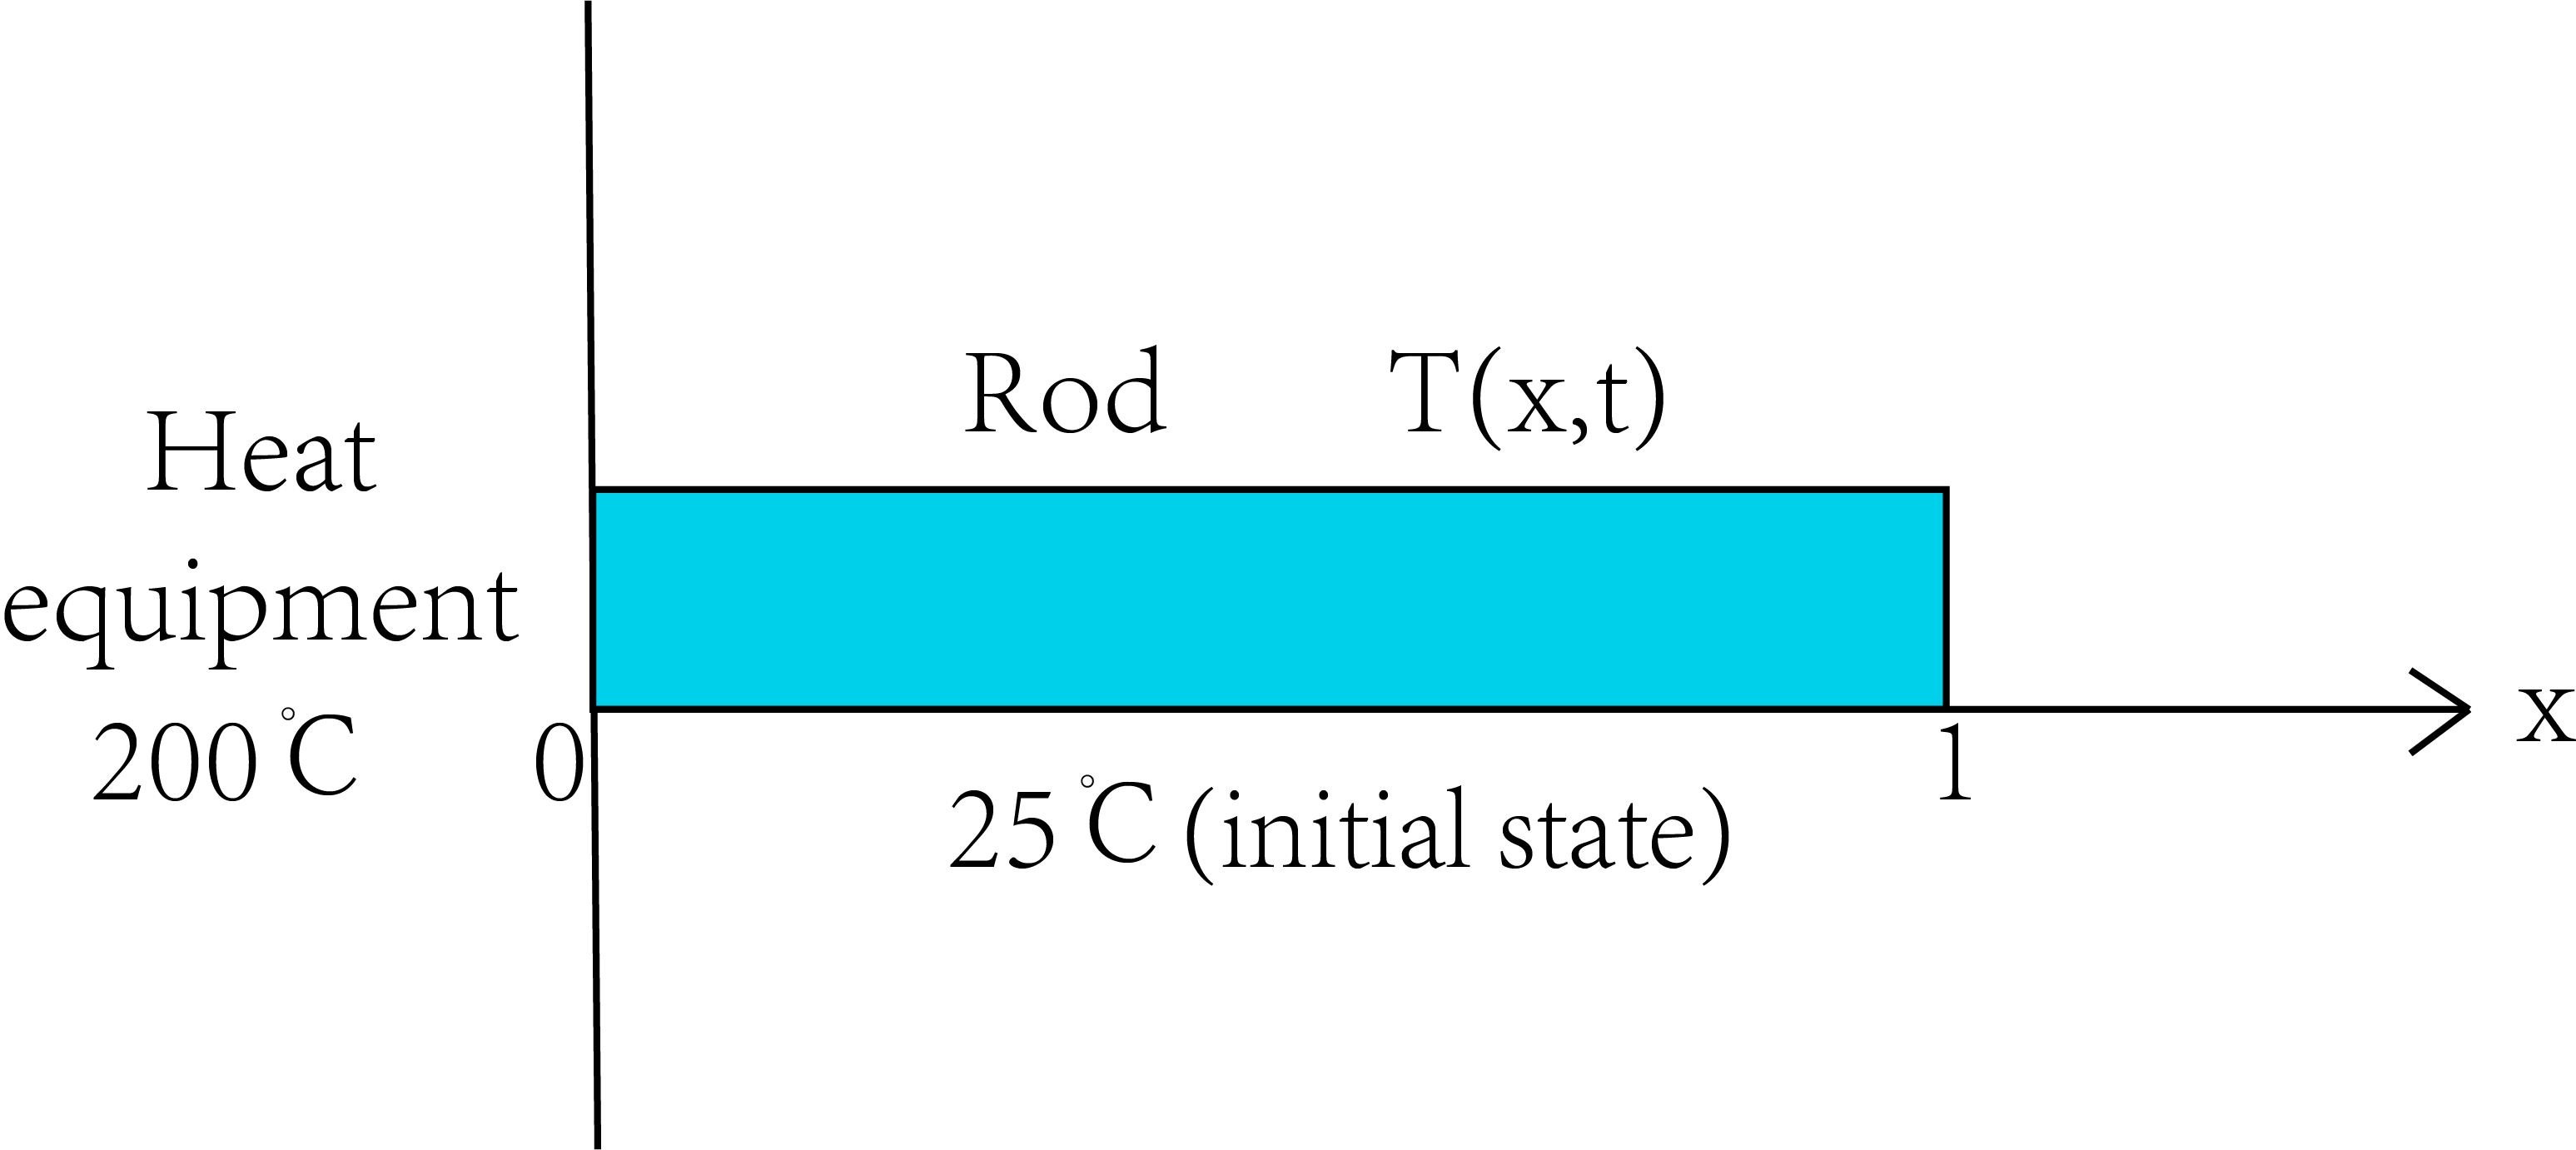
\includegraphics[width=8cm]{Figures/Heat1D_model.png}       
	\caption{The heated rod system, with the temperature at any point given by $T(x,t)$ }
	\label{Heat1D_model.fig}
\end{figure}

Our system is comprised of a rod fixed to a heated wall kept at constant temperature. The length of the rod is arbitrarily taken as 1m. The initial temperature of the rod is in equilibrium with the ambient temperature at 25$^{\circ} $C and the temperature of the wall is 200$^{\circ} $C.  We represent temperature at a point on the rod at some time with the function $T(x,t)$. Note that the rod is thin with respect to its length, thus is modeled as a 1D system, that is, temperature is solely a function of rod position and time. The goal of this simulation is to show the variations in temperature of various points on the rod over time. 

We take our initial state as:
\begin{itemize}
	\item $T(0,t)=200 ^{\circ}$C
    \item $T(x,t)=25 ^{\circ}$C, $x\ne 0$
\end{itemize}

\noindent The partial differential equation of the 1D heat propagation:
\begin{equation}
 \frac{\partial T}{\partial t} = \alpha \frac{\partial^2 T}{\partial x^2}
\end{equation}
\noindent We explicitly state that $u(\cdot)$ is a function of $x$ and $t$
\begin{equation}
 \frac{\partial} {\partial t}T(x,t) = \alpha \frac{\partial^2}{\partial x^2}T(x,t)
\end{equation}
\noindent We use a finite difference approximation to get compute the derivatives in space and time
\begin{equation}
\frac{T_{i}^{N+1}-T_{i}^{N}}{\Delta t} =\alpha\frac{T_{i+1}^{N}-2T_{i}^{N}+T_{i-1}^{N}}{\Delta x^2}
\end{equation}

\noindent Rearranging we reach the final form we need for our Forward Euler approximation. Note that the quantity $\alpha\frac{\Delta t}{\Delta x^2}$ is Fourier's number, with $\alpha$ being the thermal diffusivity of a material. In the following simulations, we arbitrarily choose Aluminium with $\alpha = 9.7e-5$.

\begin{equation}
T_{i}^{N+1}=T_{i}^{N}+\alpha\frac{\Delta t}{\Delta x^2}\big[ {T_{i+1}^{N}-2T_{i}^{N}+T_{i-1}^{N}}\big]
\end{equation}

\paragraph{Implementation}
We provide an implementation in Matlab. 

\begin{lstlisting}[language=Matlab, caption=Forward Euler and Plotting in MATLAB]

  % Values arbitrarily chosen. It's a useful exercise to vary these and look at the results
  T_final = 300;
  N_t = 2000;
  X_final = 1;
  N_x = 100;
  
  % Calculate time and x steps based on sampling size and # of samples
  T = linspace(0, T_final, N_t+1);
  X = linspace(0, X_final, N_x+1);
  dt = T(2) - T(1);  % Calculate delta t
  dx = X(2) - X(1);  % Calculate delta x

  alpha = 9.7e-5; % Thermal diffusivity of Aluminium in m^2/s
  Fo = (alpha*dt)/(dx^2); % Fouriers number = diffusive transport rate/storage rate
 
  % Define your initial condition here. This could be some function IC(x),
  %  however for simplicity's sake we take a rod with a uniform temperature
  %  and in contact with a hot plate at one end
  wall_temp = 200;
  init_temp = 25;
  
  % Initialize the N state and the N-1 state
  u_old = zeros(1, N_x+1); 
  u_old(:) = init_temp;
  u_old(1) = wall_temp;
  u_cur = u_old;
  u_plot = u_old;

  for t = 1:N_t
     for i = 2:N_x
     	 % Forward Euler solution to heat equation
         u_cur(i) = Fo*(u_old(i+1) - 2*u_old(i) + u_old(i-1)) + u_old(i);
     end
     u_cur(1) = wall_temp; % Set the left boundary to be our high of 200 
     u_old(:) = u_cur; % We move to the next time step, reset N-1 state
     u_plot = [u_plot; u_cur];
  end

  [X_plot,T_plot] = meshgrid(X,T); % Create 2D meshgrid to create surface plot

  surf(X_plot,T_plot,u_plot,'EdgeColor','none') % Create surface plot
  c = colorbar; % Attach colour bar and create scale
  c.Label.String = 'Temperature [C]';

  xlim([0 1]) % Add axis limits
  xlabel('Distance along rod [m]'); % Add descriptive axis labels
  ylabel('Time [s]');
  zlabel('Temperature [C]')

\end{lstlisting}


 \paragraph{Results}
\noindent We can create plots of the rods temperature as a function of time and position. This gives us insight into how the system evolves as we maintain our constant temperature. 
\begin{figure}[htb]
	\centering
	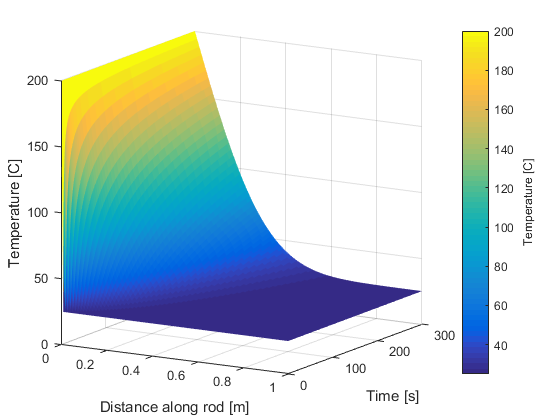
\includegraphics[width=10cm]{Figures/Heat1D_1m.png}       
	\caption{Temperature variation for the whole rod over 300 seconds}
	\label{Heat1D_1m.fig}
\end{figure}

\begin{figure}[htb]

	\centering
	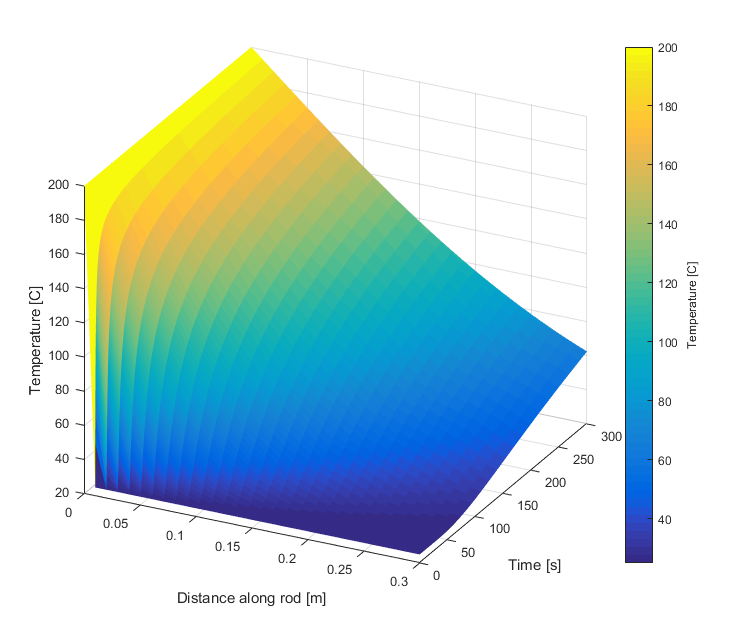
\includegraphics[width=9cm]{Figures/Heat1D_0_3m.png}       
	\caption{Temperature variation for the rod segment with x varies from 0 to 0.3m over 300 seconds}
	\label{Heat1D_0_3m.fig}
\end{figure}
\clearpage
\begin{figure}[!htb]
	\centering
	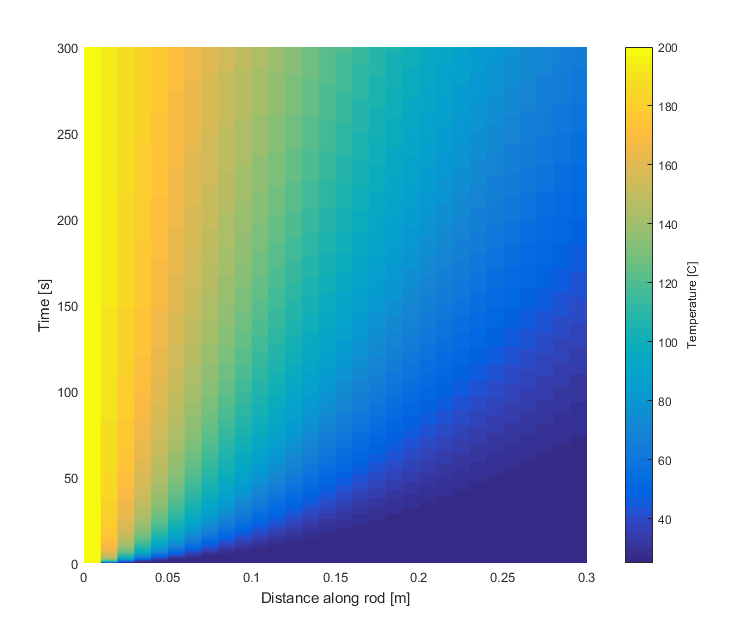
\includegraphics[width=9cm]{Figures/Heat1DTop.png}       
	\caption{Top view of the temperature variation for the whole rod over 300 seconds}
	\label{fig:Heat1D_top}
\end{figure}
 
\paragraph{Interpretation}
The results we obtain are consistent with our model and the physical characteristics. We can see that from the visualization the temperature varies in a logarithmic manner, which is 
consitent with the fact that the Forward Euler scheme approximates the exact mathematical solution to the 2nd order PDE, which takes the form of an exponential. The exact rate at which heat moves through the rod is 
dependent on the thermal conductivity of the material, which makes up part of the exponent (i.e. $e^{-m}$), thus governing the rate. 
We can see pathlines of the heat front evolve over time, especially when looking 
at the system from above. Given enough time, the rod will reach a steady state, which in this example would have the rod rest at a completely uniform temperature, since we have not incorporated any form of heat losses or sinks in the system.

 \paragraph{Conclusion}
Here we have learned that in examining systems such as the heated rod, we can safely analyze it as a 1D system. We were able to discretize the partial differential equations and 
apply a forward Euler simluation to yield phyiscally relevant and meaningful simulations. Through the Matlab visualization, we gain a better understanding of how heat is moving 
through the rod and the system. From the resources and analysis provided, it is trivial to create other initial/boundary conditions and repeat the simulations to garner a deeper
insight into the heat behaviour. This is left as an exercise to the reader. 
 


\subsection{1D vibrating string simulation}
% ***********************************************************************************
% Pure LaTeX part to be inserted in a document (be careful of depencies of packages & commands
% Prepared by XXX and YYY under the supervision of Arnaud de La Fortelle
% Fall 2017
% 2D wave propagation subsection of the modeling part
% ***********************************************************************************

\subgroup{2}{Ruitong Zhu and Qingan Zhao}

\paragraph{Model presentation}
This part is to simulate the vibrating string (i.e., 1D wave equation) and present its displacement with a time-varying image. The string held stationary at both ends and free to vibrate transversely subject only to the restoring forces due to tension in the string. $Figure 1$ shows coordinates and definies symbols for the transverse vibrating string. 

\begin{figure}[htb]
	\centering
	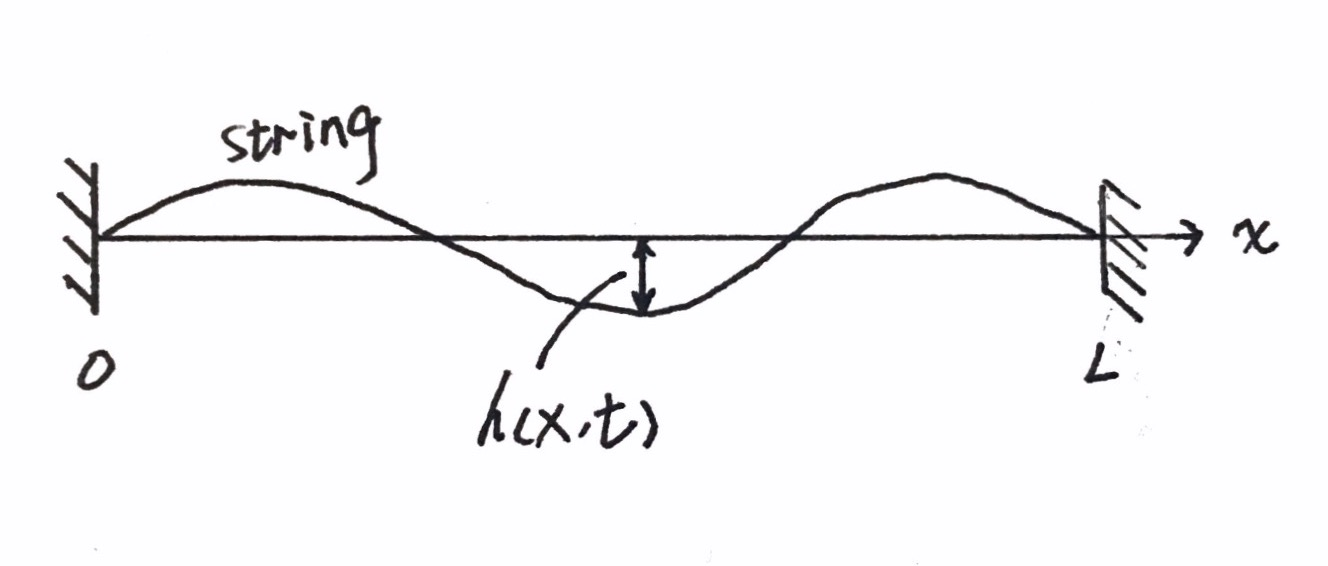
\includegraphics[width=10cm]{string.jpg}       
	\caption{Vibrating String}
\end{figure}

The partial differential equation (PDE) of this problem is given as follow:

\begin{equation}
	\frac{\partial^2 h}{\partial t^2}=a^2\left(\frac{\partial^2 h}{\partial x^2}\right)
\end{equation}

where $h$ is the wave function $h(x,t)$, representing the displacement of the string at position $x$ and time $t$; $a$ is the wave speed which equals to $\sqrt{E/\rho}$.

\paragraph{Implementation}

The simluation is based on Finite Difference Method (FDM). Using second-order central difference at time $t_n$ and position $x_i$, we can get the recurrence equation as follow:

\begin{equation}
\frac{u_{i}^{N+1}-2u_{i}^{N}+u_{i}^{N-1}}{\Delta t^2} = a^2\frac{u_{i+1}^{N}-2u_{i}^{N}+u_{i-1}^{N}}{\Delta x^2}
\end{equation}

Assume the wave speed $a = 1$; the length of the string $L$ is $2$; the maxium time for this simulation is $4$; stepsize $\Delta x$ and $\Delta t$ are both equal to $0.01$. The initial condition and the boundary condition are described as follows:
\begin{eqnarray}
h(x,0)&=&sin(\pi x)\\
\frac{\partial h}{\partial t}\bigg |_{(x,0)}&=&0\\
h(0,t)&=&h(2,t)=0
\end{eqnarray}

Here we offer the implementation in Python:

\begin{python}
	## parameter
	a = 1  ## a coefficient of stiffness
	L = 2  ## The string is constrained at x=0 and x=L.
	T = 4  ## maxium time for this simulation.
	dx = 0.01  ## time step
	dt = 0.01  ## distance step
	N = int(L/dx);
	M = int(T/dt);
	r = (a*dt/dx)**2  ## a parameter

	## initial shape of the string
	def initial(x):
	tmp = math.sin(math.pi*x)
	return tmp
	
	## initial speed of the string
	def speed(x):
	tmp = 0
	return tmp
	
	## Define an array and a blank matrix for later use.
	x = [0]
	h = np.zeros((M+1, N+1))
	
	## t=0, initial condition
	for i in range(N):
	x.append(x[i] + dx)  ## x axis
	h[0,i+1] = initial(x[i+1])  ## displacement of the string
	
	## t=dt, the first itertaion
	for i in range(N-1):
	h[1,i+1] = h[0,i+1] + r* (h[0,i] + h[0,i+2] - 2*h[0,i+1])/2 + dx*speed(x[i+1])
	## displacement of the string
	
	## t=n*dt where n>1
	for j in range(1, M):
	for i in range(N-1):
	h[j+1,i+1] = (h[j,i+2]+h[j,i]-2*h[j,i+1])*r-h[j-1,i+1]+2*h[j,i+1]
	## displacement of the string
	
	t = [0]
	for j in range(M):
	t.append(t[j] + dt)  ## t axis
	
	## Plot the 3D figure.
	fig = plt.figure()
	ax = Axes3D(fig)
	X, T= np.meshgrid(x,t)
	ax.plot_surface(X, T, h, cmap='rainbow')
	ax.set_xlabel('X')
	ax.set_ylabel('T')
	ax.set_zlabel('h')
	plt.show()
	
	## Plot the shape of string at different time
	for i in range(4):
	plt.xlabel(u'x',fontsize=14)
	plt.ylabel(u'h',fontsize=14)
	plt.show()
\end{python}

\paragraph{Results}

The dynamic change of the string is shown in $Figure 2$, ranging from $0\sim 4$.

\begin{figure}[htb]
	\centering
	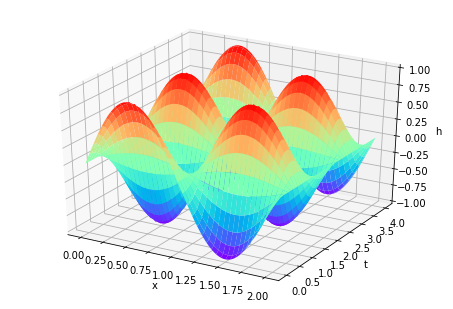
\includegraphics[width=10cm]{string3d.png}       
	\caption{Time-varying Image of the string}
\end{figure}

More specifically, the shapes of the string at different times are shown below:

\begin{figure}[ht]
	\centering
	\begin{minipage}{8cm}
		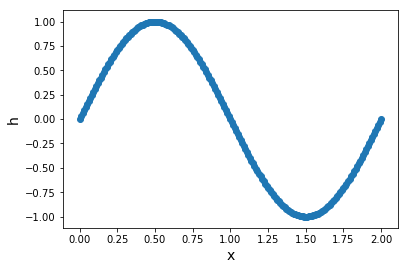
\includegraphics[width=7cm]{string0.png}   
		\caption*{t=0}
		\end{minipage}    
	\begin{minipage}{8cm}
		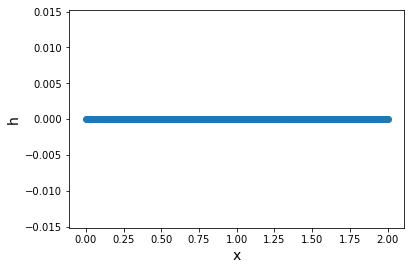
\includegraphics[width=7cm]{string0_5.png}   
		\caption*{t=0.5}
	\end{minipage}  

    \begin{minipage}{8cm}
    	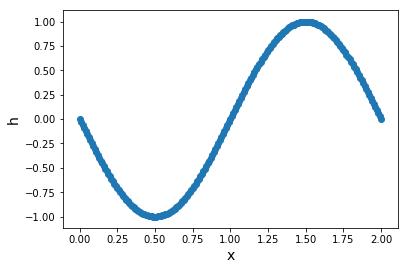
\includegraphics[width=7cm]{string1.png}   
    	\caption*{t=1}
        \end{minipage}  
    \begin{minipage}{8cm}
    	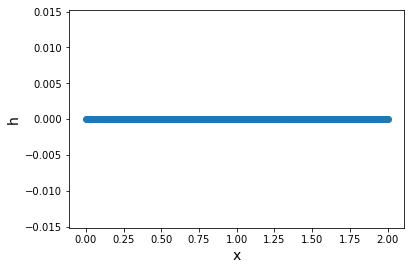
\includegraphics[width=7cm]{string1_5.png}  
    	\caption*{t=1.5} 
    \end{minipage}  
	\caption{Shape of the string at time t}
\end{figure}



\paragraph{Interpretation}

The results are consistent with our expectation. The shape of the string depends on the initial and boundary conditions. In this case, the string is in the shape of a sine wave that changes periodically. 

The initial and boundary conditions can be changed easily at the code by modifying the function $initial()$ and $speed()$. Readers can plot more complicated image with different initial displacement and speed function.

\paragraph{Conclusion}
Finite Difference Method is a practical method to obtain the numerical solution of a Partial Differential Equation. We can learn that it is applicable for one dimentional problems like 1D wave equation and 1D heat equation. It's not difficult to understand but there are some places worth special attention while writing the code. For example, the first iteration needs to be distinguished from other iterations since $t_{N-1}$ is not defined. 



\subsection{1D traffic simulation}
% ***********************************************************************************
% Pure LaTeX part to be inserted in a document (be careful of depencies of packages & commands)
% Prepared by XXX and YYY under the supervision of Arnaud de La Fortelle
% Fall 2017
% 1D LWR traffic model of the simulation part
% ***********************************************************************************

\subgroup{3}{Yue Hu and Carlin Yao}

\paragraph{Model presentation}
What is the model we want to simulate? What do we want to observe? Which is the state space and the dynamics?

\paragraph{Implementation}
Explain the structure of the code. Do not put necessarily all the code (not more than 100 lines) since some routines (functions) can hide efficiently some unnecessary complexity. Provide a code that run (and explicit librairies and dependencies). Ensure your file name is aligned with this part.

 \paragraph{Results}
 Explain the quantities you are studying (i.e. metrics and statistics). Provide good visualization.
 
\paragraph{Interpretation}
Relate these quantities to the model and to theoretical knowledge of the course.

 \paragraph{Conclusion}
 What have we learned? Is everything aligned (theory and practice)? What was difficult? Provide perspectives.
 


\subsection{Random walk in 2D simulation}
% ***********************************************************************************
% Pure LaTeX part to be inserted in a document (be careful of depencies of packages & commands)
% Prepared by XXX and YYY under the supervision of Arnaud de La Fortelle
% Fall 2017
% 12 random walk subsection of the simulation part
% ***********************************************************************************

\subgroup{4}{Yue Hu, Carlin Liao and Robert Ruigrok}

\paragraph{Model presentation}
In this example we simulate the random walk of a particle in a 2D space. A random walk is a mathematical object, known as a stochastic or random process, that describes a path that consists of a succession of random steps. In order to simulate this process, we let a particle move over a discretized grid where its motion is drawn from a set of possible directions. In this simulation we are interested in finding expected distribution of particles after a certain number of time steps as well as the position where they hit the boundaries of the spatial grid.\newline

A particle starts at a specified initial position, from where it begins moving through the grid. In our code, we used a coordinate system to represent the location of a particle as provided in figure \ref{fig:RandomWalkGrid}. The outer border of the grid is enclosed by a ``wall''. When the particle hits this wall, its motion stops and the location where it makes contact is registered.

\begin{figure}[htb]
    \label{fig:RandomWalkGrid}
	\centering
	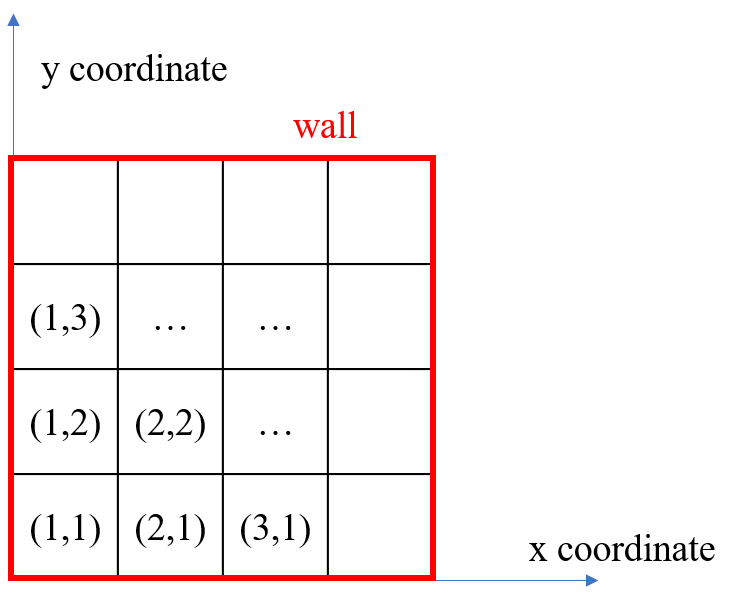
\includegraphics[width=6cm]{RandomWalkGrid.png}       
	\caption{Coordinate representation in spatial grid}
\end{figure}

The dynamics of a particle are relatively straightforward and can be described by equation \ref{eq:RandomWalkDynamics}. A particle has 5 options for its motion: moving up, right, down, left or no motion (options are depicted in figure \ref{fig:RandomWalkMotion}). Every motion has a certain probability $p$ to occur. These probabilities can be given as input and must add up to 1.

\begin{equation}
\label{eq:RandomWalkDynamics}
X_{k+1}(x,y) = X_k(x,y) +  \begin{cases}
(0,1) &\text{with probability $p\uparrow$}\\
(1,0) &\text{with probability $p\rightarrow$}\\
(0,-1) &\text{with probability $p\downarrow$}\\
(-1,0) &\text{with probability $p\leftarrow$}\\
(0,0) &\text{with probability $p\ \bullet$}
\end{cases}
\end{equation}



\begin{figure}[htb]
    \label{fig:RandomWalkMotion}
	\centering
	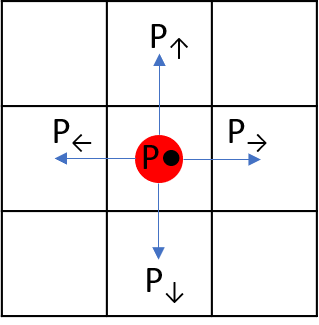
\includegraphics[width=3cm]{RandomWalkMotion.png}       
	\caption{Potential motion per time step}
\end{figure}


\paragraph{Implementation} 
At the top of the file, it is possible to set the grid size, starting position of particles, \# of particles, simulation horizon and motion direction probabilities. The script will also generate snapshots of the particle distribution at different moments in time during the simulation. By selecting the number of subplots, you can determine how many instances you would like to see. This will provide insights into how the particle distribution develops over time. \newline

Particles are simulated one at a time. The simulation runs until the time horizon $T$ is reached or the particle hits the wall. Their position is saved in a 3-dimensional array (time, x-position, y-position) at specified moments in time only; this way the amount of required memory is kept to a minimum. %You do not save the position of every particle at every time step, but you only ``count'' their positions at time steps that you are interested in. Information about individual particles gets lost, but that is fine.
\newline

Information about where particles hit the wall is included in the same arrays. This data ``circumvents'' the $n \times n$ data about the particle distribution within the grid. As a result, when we plot the full array we can see the distribution of particles in the grid at their respective location, and the distribution of particles at the wall directly ``behind'' the wall.\newline

\begin{python}
# This file will model/simulate the random motion

import numpy as np
import matplotlib.pyplot as plt
from random import *
import pylab

############## START INPUT #################

GridSizeSquare = 20 # n, will create an nxn grid
#define starting position as ratio or grid size
Pos_init = np.ceil(np.array([0.4,0.4])*GridSizeSquare)
#T is the total amount of time steps, scale with square of grid size. 0.3 is nice
T = 0.3*np.power(GridSizeSquare, 2)
n_particles = 10000 # #particles. 10000+ recommended
# define the # of subplots for intermediate time snap shots
subplot_row = 2             
subplot_column = 2
#defines the drift probabilities: ([up,right,down,left,0]) 
motion_prob = np.array([0.2,0.2,0.2,0.2,0.2])

############## END INPUT #################

#only look at square grids, but this could be changed:
x_grid = GridSizeSquare
y_grid = GridSizeSquare
n_subplot = subplot_row*subplot_column
Plot_interval = np.floor((T-1)/(n_subplot-1))
#This determines when you take snapshots of the process, every "Plot_interval" time steps

# now define the probabilities of the random walk
# notation of motion ([up,right,down,left,no motion])
# I normalized in case probabilities do not add up to 1...
motion_prob = motion_prob/np.sum(motion_prob)
# define the change in coordinates of every motion:
motion_xy = np.array([[0,1],[1,0],[0,-1],[-1,0],[0,0],])
motion_prob_percentile = np.cumsum(motion_prob)
# this is used later to draw from with randomizer

# make an empty data grid from where you are going to count the amount occurrences and hits against the wall
Data = np.zeros((x_grid+2,y_grid+2)) # "+2" for wall data
Data_resized = np.zeros((Data.shape[0]+1,Data.shape[1]+1))
# This for plotting purposes, I need to add an extra row an column for some reason
# Now create a new empty data set for the intermediate plots:
Data_TimeVarying = np.zeros((n_subplot,Data_resized.shape[0],Data_resized.shape[1]))

# construct some arrays for plotting later on:
xx, yy = pylab.meshgrid(
    pylab.linspace(-1,x_grid+1,x_grid+3),
    pylab.linspace(-1,y_grid+1,y_grid+3))

# Here, start loop over all the particles after each other:
for i in range(1, n_particles+1):
    # Initialize simulation
    t = 0
    HitWall = False
    Pos = Pos_init
    Subplot = 1
    
    # start simulation
    while t < T and not HitWall:
                
         # Now continue with the motion simulation
        MotionRandom = random()
        IndexMotion = np.argmax(motion_prob_percentile>MotionRandom)
        Pos = Pos + motion_xy[IndexMotion,:] #this works
        
        # Now check for hitting the wall
        if Pos[0] == 0 or Pos[1] == 0 or Pos[0] == x_grid+1 or Pos[1] == y_grid+1:
            if Subplot <= n_subplot:             
                Data_TimeVarying[Subplot-1,Pos[0],Pos[1]] = Data_TimeVarying[Subplot-1,Pos[0],Pos[1]]+1
            HitWall = True

        # Now record the position for time dependent plotting purposes
        if t % Plot_interval == 0 and Subplot <= n_subplot and not(HitWall):   #so create a subplot every Plot_interval time steps
            Data_TimeVarying[Subplot-1,Pos[0],Pos[1]] = Data_TimeVarying[Subplot-1,Pos[0],Pos[1]]+1
            Subplot = Subplot+1        
        
        t = t+1
    
    
    #This was basically the whole simulation, now save the results
    Data[Pos[0],Pos[1]] = Data[Pos[0],Pos[1]] + 1
    # I need to give resize Data with an extra row and column, since pcolor doesn't plot the full range of the matrix...
    Data_resized[:-1,:-1] = Data       


# Now I need to do some post-processing of the intermediate measurements.
# I need to add the particles that hit the wall in earlier time steps to the 
# later plots, so the total amount of particles is always n  
Data_TimeVarying_Corrected = np.cumsum(Data_TimeVarying,axis=0)
Data_TimeVarying_Corrected[:,1:x_grid+1,1:y_grid+1] = Data_TimeVarying[:,1:x_grid+1,1:y_grid+1]


# This loop creates subplots at several time instances
plt.figure()
for j in range(1, n_subplot+1):
    #Now visualize the outcomes
    pylab.subplot(subplot_row, subplot_column, j)
    pylab.pcolor(xx,yy,np.transpose(Data_TimeVarying_Corrected[j-1,:,:]))
    TitleString = 'Distribution at t = ' + str((j-1)*Plot_interval+1)
    pylab.title(TitleString)
    # and a color bar to show the correspondence between function value and color
    pylab.colorbar()
    pylab.hold(True)
    pylab.plot([0, x_grid],[0, 0], 'r',[0, x_grid],[y_grid, y_grid], 'r',[0, 0],[0, y_grid], 'r',[x_grid, x_grid],[0, y_grid], 'r')
    pylab.plot(Pos_init[0]-0.5,Pos_init[1]-0.5,'ro')

pylab.show()

# This plot shows the final distribution, including distribution along the walls
plt.figure()
pylab.pcolor(xx,yy,np.transpose(Data_resized))
pylab.title('Final distribution at t = %d, including hitting walls' %T)
# and a color bar to show the correspondence between function value and color
pylab.colorbar()
pylab.hold(True)
pylab.plot([0, x_grid],[0, 0], 'r',[0, x_grid],[y_grid, y_grid], 'r',[0, 0],[0, y_grid], 'r',[x_grid, x_grid],[0, y_grid], 'r')
pylab.plot(Pos_init[0]-0.5,Pos_init[1]-0.5,'ro')
pylab.show
\end{python}



\paragraph{Results}
In this section we included two simulation for both a $10x10$ grid and a $20 \times 20$ grid, with a different simulation time horizon $T$. Both simulations use 10,000 particles and have a motion probability of $0.2$ in all directions. \newline

It is clearly visible how the particles spread out over time and make their way to the walls over time. The more particles that are simulated per grid resolution, the smoother the distribution becomes. You can clearly see that 10,000 particles simulated lead to a clean distribution in the smaller plot of figure \ref{fig:RandomWalk10}, while the larger plot of \ref{fig:RandomWalk20} shows a more grainy distribution.

\begin{figure}[htb]
    \label{fig:RandomWalk10}
	\centering
	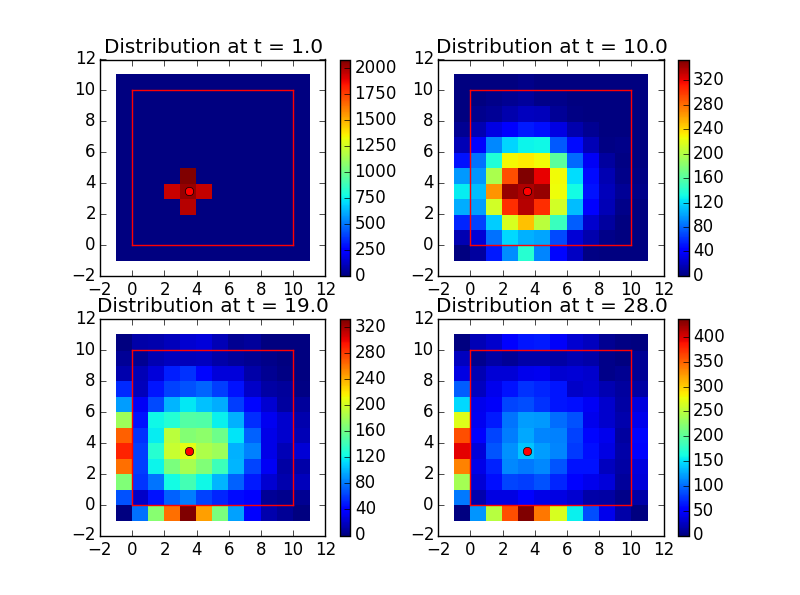
\includegraphics[width=14cm]{figure10x10.png}       
	\caption{Particle distribution for $10 \times 10$ grid at different time steps}
\end{figure}

\begin{figure}[htb]
    \label{fig:RandomWalk20}
	\centering
	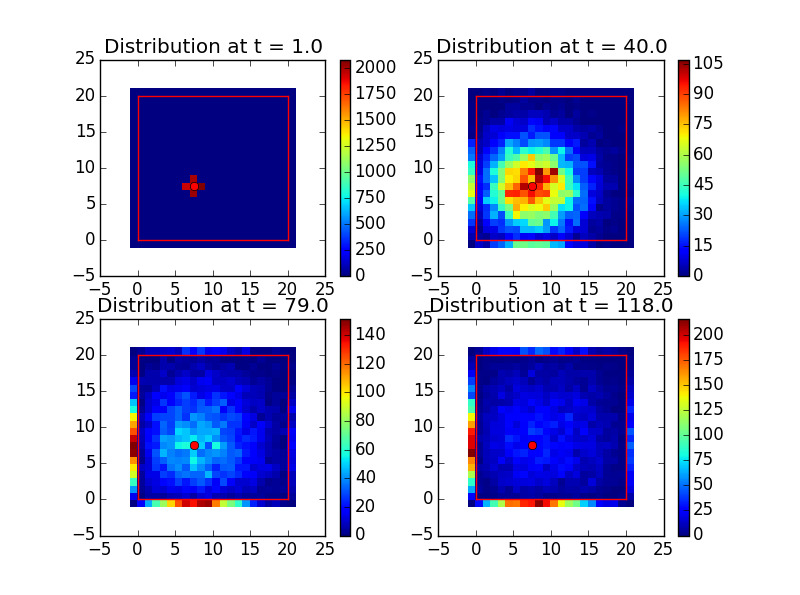
\includegraphics[width=14cm]{figure20x20.png}       
	\caption{Particle distribution for $20 \times 20$ grid at different time steps}
\end{figure}


 
\paragraph{Interpretation}
{\it Relate these quantities to the model and to theoretical knowledge of the course.}\newline

{\it I think this motion is described by Fick's Law in 2 dimension. The concentration on a specific point changes over time, depending on the concentration of its surroundings. Should we derive why the second derivative matters? $\phi$ is the concentration, $D$ the diffusion coefficient.}

\begin{equation}
\label{eq:FicksLaw}
\frac{d\phi}{dt} = D\nabla\phi = D \big(\frac{d^2\phi}{dx^2} + \frac{d^2\phi}{dy^2}\big)
\end{equation}


 \paragraph{Conclusion}
 \textit{What have we learned? Is everything aligned (theory and practice)? What was difficult? Provide perspectives.}
 
 The dynamics of the random walk were easy to model. The challenge in this simulation was to save the data for the intermediate time steps. Since the particles are simulated one by one for the full time horizon, we had to write some non-intuitive code to save the location of every particle at the relevant intermediate time steps. \newline
 
 From the lecture we recall that diffusion distance scales with the square root of time. Here we tried to simulate that. When doubling the grid size and taking a four times higher simulation horizon, the distribution looks similar. However, we have the idea that the scaling did not work for 100\%. At the end of the scaled simulation horizon, it seems as if the smaller grid has relatively more particles in the grid than the larger grid has. What could cause this difference?
 
